\documentclass{standalone}
\usepackage{tikz}
\usepackage{ctex,siunitx}
\usepackage{tkz-euclide}
\usepackage{amsmath}
\usetikzlibrary{patterns, calc}
\usetikzlibrary {decorations.pathmorphing, decorations.pathreplacing, decorations.shapes,}
\begin{document}
\small
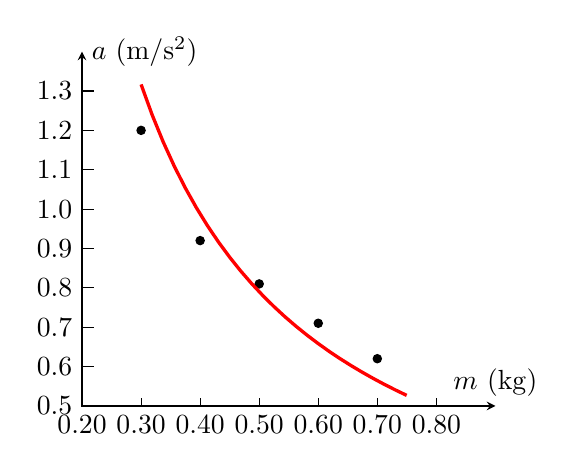
\begin{tikzpicture}[>=stealth,xscale=7.5,yscale=5,domain=0.3:0.75]
  \draw [<->](0+0.2,.9+0.5)node [right]{$a$ (\unit{m/s^2})}--(0+0.2,0+0.5)--(.7+0.2,0+0.5)node [above]{$m$ (\unit{kg})};
  \foreach \x in {1,2,3,4,5,6}
  {
      \draw(0+0.2,\x/10+0.5) --(0.02+0.2,\x/10+0.5);
      \draw(\x/10+0.2,0+0.5)--(\x/10+0.2,0.02+0.5);
  }
  \draw(0+0.2,6/10+0.5) --(0.02+0.2,6/10+0.5);
  \draw(0+0.2,7/10+0.5) --(0.02+0.2,7/10+0.5);
  \draw(0+0.2,8/10+0.5) --(0.02+0.2,8/10+0.5);
  \draw [fill=black] (0.3  ,  1.2)  circle(.2pt and 0.3pt);%[radius=.3pt and 0.2pt];
  \draw [fill=black] (0.4  , 0.92)  circle(.2pt and 0.3pt);%[radius=.3pt and 0.2pt];
  \draw [fill=black] (0.5  , .81 )  circle(.2pt and 0.3pt);%[radius=.3pt and 0.2pt];
  \draw [fill=black] (0.6  ,  .71)  circle(.2pt and 0.3pt);%[radius=.3pt and 0.2pt];
  \draw [fill=black] (0.7  ,  .62)  circle(.2pt and 0.3pt);%[radius=.3pt and 0.2pt];
  \draw[color=red, very thick] plot (\x,.395/\x ) ;
  \node at (0+0.2,0+0.5)[below]{0.20};
  \node at (0.1+0.2,0+0.5)[below]{0.30};
  \node at (0.2+0.2,0+0.5)[below]{0.40};
  \node at (0.3+0.2,0+0.5)[below]{0.50};
  \node at (0.4+0.2,0+0.5)[below]{0.60};
  \node at (.5+0.2,0+0.5)[below]{0.70};
  \node at (.6+0.2,0+0.5)[below]{0.80};
  \node at (0+0.2,0+0.5)[left]{0.5};
  \node at (0+0.2,0.1+0.5)[left]{0.6};
  \node at (0+0.2,0.2+0.5)[left]{0.7};
  \node at (0+0.2,0.3+0.5)[left]{0.8};
  \node at (0+0.2,0.4+0.5)[left]{0.9};
  \node at (0+0.2,.5+0.5)[left]{1.0};
  \node at (0+0.2,.6+0.5)[left]{1.1};
  \node at (0+0.2,.7+0.5)[left]{1.2};
  \node at (0+0.2,.8+0.5)[left]{1.3};
\end{tikzpicture}
\end{document}